\documentclass[a4paper,UTF8]{ctexart}

\usepackage{amsmath, amsthm, amssymb, amsfonts, hyperref, mathrsfs}%美国数学学会的包+?
\usepackage{geometry} %控制界面
\usepackage{bookmark}
\usepackage{fancyhdr} % header & footer
\usepackage{appendix} % 附录
\usepackage{tikz} %作图
\usepackage{graphicx} %插入图片的宏包
\usepackage{float} %设置图片浮动位置的宏包
%\usepackage{subfigure} %插入多图时用子图显示的宏包
\usepackage{listings} %引用代码
\usepackage{physics,mathtools} %物理数学工具
\usepackage{comment}
\usepackage{framed}
\usepackage{caption}
\usepackage{subcaption}
\geometry{top=2.5cm,bottom=2.5cm,left=2.5cm,right=2.5cm} % 布局要求
\pagestyle{fancy} % fancy分格
\fancyhf{} % 清除所有页眉页脚
\renewcommand\headrulewidth{0.6pt}
\renewcommand\footrulewidth{0.6pt}
% font
\setCJKmainfont{Noto Serif CJK SC}[BoldFont={Noto Serif CJK SC Bold}, ItalicFont=]
\lhead{何金铭 PB21020660$\mid$座位号:8}
\cfoot{纠缠光子的制备及性质预习报告}
\rhead{\thepage}
\lfoot{2024.4.28}
\rfoot{USTC}
%\bibliographystyle{plain} % 引用样式
\everymath{\displaystyle} % display
%============================================================

\begin{document}

\begin{center}
    \textbf{\Large 纠缠光子的制备及性质预习报告}
    \par \text{\large 何金铭 PB21020660}
\end{center}

\section{实验目的}

本实验系统基于准相位匹配PPKTP晶体的参量下转换过程, 结合Sagnac干涉环结构, 制备出高质量的偏振纠缠光子源, 其所具有的高亮度、高稳定性等特性适用于远距离的量子保密通信、量子隐形传态等诸多方面.

\begin{enumerate}
    \item 了解量子叠加态和纠缠态的基本原理和性质,理解Bell不等式和CHSH不等式
    \item 了解基于准相位匹配PPKTP晶体产生纠缠光子对的原理, 学习操作和使用量子光学实验中的基本器件;简要了解光纤传输和耦合的理论和技术和单光子测量技术
    \item 学习光子纠缠对比度的符合测量方法, 并实验验证Bell不等式
    \item 观测纠缠态的量子特性, 并体会其和经典物理现象的区别
\end{enumerate}

\section{实验原理}

\subsection{量子比特}

qubit的态可表示为:

\begin{equation}
    \ket{\psi} = \alpha \ket{0} + \beta \ket{1} = \alpha \ket{H} + \beta\ket{V} (photon)
\end{equation}

量子态具有相干性。

\subsection{纠缠态}

纠缠态是量子系统的一种特性,以一个常见的Bell态为例:

\begin{equation}|\Psi^-\rangle_{AB}=\frac{1}{\sqrt{2}}\big(|HV\rangle_{AB}-|VH\rangle_{AB}\big)\end{equation}

为了说明这样一个状态在实验上所展现出的性质, 这里首  先引入符合测量的概念. 这里我们的系统包含两个光子, 假设这两个光子分别发送给了Alice和Bob, 他们分别让光子通过特定角度的偏振片, 之后进入探测器. 当Alice和Bob手中的探测器分别输出了一个脉冲信号, 且这两个脉冲信号落入同一个时间窗口(这时认为这两个脉冲信号是同时产生的), 则称产生了一个符合计数, 而这个测量的过程则成为符合测量

但实际情况下量子态有误差,除了HV和VH的符合计数外,还有HH和VV的计数,这些计数的比例一般会小于符号计数。

检测这个Bell态$|\Psi^-\rangle_{AB}$可以于$\big( |+\rangle_{A},|+\rangle_{B},|-\rangle_{A},|-\rangle_{B}\big)$这组正交基矢下展开

\begin{equation}\begin{aligned}
\left|\Psi^{-}\right\rangle & =\frac{1}{\sqrt{2}}\left(|H\rangle_{A}|V\rangle_{B}-|V\rangle_{A}|H\rangle_{B}\right) \\
&=\frac{1}{2\sqrt{2}}\left[\left(\left|+\right\rangle+\left|-\right\rangle\right)_{A}\left(\left|+\right\rangle-\left|-\right\rangle\right)_{B}-\left(\left|+\right\rangle-\left|-\right\rangle\right)_{A}\left(\left|+\right\rangle+\left|-\right\rangle\right)_{B}\right] \\
&=\frac{1}{\sqrt{2}}\left(\left|-\right\rangle_{A}\left|+\right\rangle_{B}-\left|+\right\rangle_{A}\left|-\right\rangle_{B}\right).
\end{aligned}\end{equation}

 这时我们发现,理想情形下,我们只有在基矢$|+-\rangle_{AB}$ 和$|-+\rangle_{AB}$下才能测得的符合计数,而无法观察到基矢$|++\rangle_{AB}$和$|--\rangle_{AB}$下的符合计数,这便是量子相干性在实验中所体现出的重要现象,而这也正是纠缠态核心的性质之一.

从上述结果可以看出,在特定的测量基矢下,处于纠缠态的两个粒子能够展现出关联性质,这种性质是一种非经典关联.实验上我们用极化关联曲线来描述纠缠双方用不同的基矢测量所反应出来的关联性质. 具体做法是,Alice 和 Bob 其中一方固定测量一个极化方向,而另一方测量 0 到 360°各个值的符合计数,从而画出一条曲线. 典型的两条极化关联曲线是 Alice 分别选定 $\mathcal{H}(0^\circ)$和$+(45^\circ)$, Bob 测量 0°到 360°所得到的曲线. Alice 分别选择测量角度为 0°和 45°时得到的关联曲线的极大值和极小值的比值即为我们之前所说的选 HV 或者+/-基矢的对比度.

\subsection{Bell不等式与CHSH不等式}

Bell不等式和CHSH不等式是为了定量检验局域实在论和量子力学的区别。

定域实在论假定:

\begin{enumerate}
    \item 物理实在:系统无干扰的情况下,如果我们能确定地预言
一个物理量的值,那么这个物理量就必定是一个客观
实在,对应着一个物理实在元素;
    \item 完备性:一个完备的理论应当包括所有的物理实在元素;
    \item 局域性:对于类空分开的、无相互作用的两系统,对其中
一个作用一定不影响另一个系统。(狭义相对论要求)
\end{enumerate}

Bell 为了能够定量分析问题,引入隐变量$\lambda$,概率分布与输入测量装置的量子态有关,为$\rho(\lambda)$,满足$\int _{\rho}\rho\left ( \lambda\right ) $d$\lambda= 1$,则对于给定的$\boldsymbol{n}$,可观测量$\boldsymbol{n}\cdot\sigma$的单次测量结果$E(\boldsymbol{n},\lambda)=\pm1$由隐变量决定,其期望值为:

$$
E(\boldsymbol{n})=\int E\left(\boldsymbol{n},\lambda\right)\rho(\lambda)\mathrm{d}\lambda 
$$
 对于一个两粒子系统同理,存在一个全局的隐变量$\lambda$,有

$$
E(\boldsymbol{e}_1,\boldsymbol{e}_2)=\int\rho(\lambda)E(\boldsymbol{e}_1,\lambda)E(\boldsymbol{e}_2,\lambda).
$$

从这样一个假设出发,引入 Bell 态$|\Psi^-\rangle$,为了与量子力学的基本结论一致,此时$E(\boldsymbol{n},-\boldsymbol{n})=-1$.在此前提下,Bell 得出结论,对于任意方向$\boldsymbol{a},\boldsymbol{b},\boldsymbol{c}$,有

$$
|E(\boldsymbol{a},\boldsymbol{b})-E(\boldsymbol{a},\boldsymbol{c})|\leq1+p(\boldsymbol{b},\boldsymbol{c}).
$$

如果量子力学正确,则该不等式可以被违背.对于态$|\Psi^-\rangle$,我们有

$$
E(\boldsymbol{e}_1,\boldsymbol{e}_2)=\langle\Psi^-|\left(\boldsymbol{e}_1\cdot\sigma\right)\otimes(\boldsymbol{e}_2\cdot\sigma)|\Psi^-\rangle=-\boldsymbol{e}_1\cdot\boldsymbol{e}_2=-\cos\left\langle\boldsymbol{e}_1,\boldsymbol{e}_2\right\rangle.
$$

若有$\boldsymbol{a}\bot\boldsymbol{b}$且$\boldsymbol{c}$与$a$间夹角为$\theta$,则 Bell 不等式左边为$\cos\theta$,而右边则是$1-\sin\theta$,于是Bell 不等式等价于$\sin\theta+\cos\theta\leq1$,显然存在$\theta$破坏该不等式.

Bell不等式虽然给出了局域实在论和量子力学的区别,但是其实验验证并不容易,因为Bell不等式的违背需要很高的精度,而且实验中存在很多误差,所以实验上往往使用CHSH不等式来验证。

下面我们采取一种最简单的方法引入 CHSH 不等式. 首先引入记号$A_1=\boldsymbol{a}_1\cdot\sigma$ 对$A_2,B_1,B_2$定义类似,这四个可观测量的可能取值均为±1. 我们考察

$$
\mathcal{B}_{\mathrm{CHSH}}=A_{1}\otimes(B_{1}+B_{2})+A_{2}\otimes(B_{1}-B_{2})
$$

通过分析可知(四个可观测量分别取$\pm1$遍历),对于每个单次测量而言,$\mathcal{B}_{\mathrm{CHSH}}=\pm2$ 则无论输入怎样的 2-qubit 态,都有$|\mathcal{B}_{\text{снsн}|\leq2}$, 即

$$
|E\left(\boldsymbol{a}_1,\boldsymbol{b}_1\right)+E\left(\boldsymbol{a}_1,\boldsymbol{b}_2\right)+E\left(\boldsymbol{a}_2,\boldsymbol{b}_1\right)-E\left(\boldsymbol{a}_2,\boldsymbol{b}_2\right)|\leq2,
$$

这就是 CHSH 不等式. 该不等式并没有假设任何具有特殊性质的量子态,对于实验而言只要我们能够制备一个两光子态,选取一定的基矢(即使存在误差), 观测到违背即可论证量子力学的正确性.

本实验中,我们利用通过 PPKTP 晶体准相位匹配产生的纠缠光子对完成 CHSH 不等式违背的验证. 实验中我们需要测量的即$E(\boldsymbol{a}_1,\boldsymbol{b}_1),E(\boldsymbol{a}_1,\boldsymbol{b}_2),E(\boldsymbol{a}_2,\boldsymbol{b}_1),E(\boldsymbol{a}_2,\boldsymbol{b}_2)$这四个可观测量(这里也可以称为关联系数), 它可以通过在两个光子路径上放入不同角度的偏振片,记录透过偏振片光子的符合计数实现. 对于$E(\boldsymbol{a}_i,\boldsymbol{b}_j),\boldsymbol{a}_i$和$\boldsymbol{b}_j$表示光子 1 和光子 2 的测量基矢方向,实验中一组测量基矢对应偏振片的两个角度$\theta$ 和$\theta^{\perp}$(本征值+1和-1), 这里将$\boldsymbol{a}_i$和$\boldsymbol{b}_j$对应的角度分别记作$\theta_{ai}$和$\theta_{bj}$.为了得到关联系数

$$
E\left(\boldsymbol{a}_i,\boldsymbol{b}_j\right)=\langle\psi|(\boldsymbol{a}_j\cdot\sigma)_1\otimes(\boldsymbol{b}_j\cdot\sigma)_2|\psi\rangle,
$$

我们需要记录四种偏振片角度组合的符合计数率,从而得到

$$
E(\boldsymbol{a}_i,\boldsymbol{b}_j)=\frac{C(\theta_{ai},\theta_{bj})+C(\theta_{ai}^\perp,\theta_{bj}^\perp)-C(\theta_{ai},\theta_{bj}^\perp)-C(\theta_{ai}^\perp,\theta_{bj})}{C(\theta_{ai},\theta_{bj})+C(\theta_{ai}^\perp,\theta_{bj}^\perp)+C(\theta_{ai},\theta_{bj}^\perp)+C(\theta_{ai}^\perp,\theta_{bj})}.
$$

其中$C(\theta_{ai},\theta_{bj})$表示两个偏振片分别为
$\theta_{ai}$和$\theta_{bj}$时的符合计数率.这里以实验中所制备出的态
$|\Psi^+\rangle_{AB}$为例,当
$\theta_{a1}=0^{\circ},\theta_{a2}=45^{\circ},\theta_{b1}=22.5^{\circ},\theta_{b2}=-22.5^{\circ}$
时,CHSH不等式左侧能够取到极大值$2\sqrt{2}$.



\subsection{PPKTP晶体准相位匹配和纠缠光子对的制备}

本实验中,我们主要利用一种二阶非线性效应产生纠缠光子对.在该过程中,入射的光子(称为泵浦光子,频率$\omega_\mathrm{p}$)会自发劈裂成两个沿与入射光子同方向传输,频率相同的低能量光子,分别称为信号(signal)光和闲频光(idler), 频率为$\omega_{\mathrm{i}}=\omega_{\mathrm{s}}=\omega_{\mathrm{p}}/2$.该过程称为共线且简并的 2 型自发参量下转换过程(Spontaneous Parametric DownConversion), 参量表示该过程能量守恒;下转换表示该过程使光子能量变低;该过程没有种子光激发,属于自发过程;2 型为 SPDC 的修饰词,表示出射的两个下转换光子偏振相互垂直.

该过程显然需满足能量守恒,除此之外,还需满足动量守恒(即相位匹配条件) $\Delta k=k_{\mathrm{p}}-k_{\mathrm{s}}-k_{\mathrm{i}}=0$,于是有$2n_{\mathrm{p}}=n_{\mathrm{s}}+n_{\mathrm{i}}$.也就是说,给定特定波长$\omega_{\mathrm{p}}$,我们需要利用各向异性介质的色散关系,在晶体中找到满足动量守恒所要求的的折射率关系的方向, 按此切割晶体.但当$\Delta k\neq0$并不意味着该过程不会发生,本质上而言,不满足相位匹配条件的能量守恒过程也会发生,但由于非线性过程在晶体内泵浦光所及之处均等概率发
生,当晶体较厚时,只有满足相位匹配条件的方向才能保证在泵浦光所经各处的 SPDC 光子干涉相长,以较大强度出射晶体. 事实上,出射光强表达式中包含如下和光栅方程的类似的一项

$$
I\propto\text{sinc}^2\frac{l\:\Delta k}2
$$

其中$l$为晶体长度.可见相位失配时,泵浦光入射后仍能产生 SPDC 光子,但随着晶体长度增加,信号光的光强呈现周期震荡,在$l\Delta k/2=\pi/2$ 时信号光达到最强,我们定义此时晶体长度为相干长度$l_\mathrm{c}$.相位匹配条件满足时,光强的表达式中震荡项消失,信号光光强随晶体长度增长而变强.

因此一般而言,我们需要按照相位匹配条件切割晶体,但还存在一种方法,在相位匹配条件不满足时仍能达到同样效果,称为准相位匹配(Quasi-Phase-Matching)


\begin{figure}[H]
    \centering
    \begin{minipage}[b]{0.9\textwidth}
        \centering
        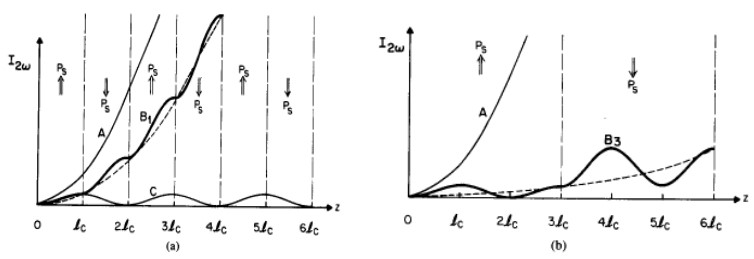
\includegraphics[width=0.9\textwidth]{./fig1.jpg}
    \end{minipage}
\end{figure}

如上图 a 所示,曲线 A 表示相位匹配的情况,此时随着作用距离的增长,信号光光强不断增加;曲线 C 表示相位不匹配的情况,此时随着作用距离的增长,信号光光强周
 期性地振荡.曲线 B 则是准相位匹配的结果,它使得信号光持续增长,但是事实上它却并没有实现相位匹配,因此称之为准相位匹配. 准相位匹配的做法是周期性地改变非线性晶体的取向,在信号光达到最强即将下降时,改变非线性极化率的符号,从而使得信号光光强继续增长,从图中可见,极化周期等于两个相干长度.图 b 每 3 个相干长度改变一次极化方向的结果,在前 3 个相干长度中,信号光的增长符合相位不匹配的情况的振荡情况.在4~6 个相干长度中,极化方向改变,信号光再次振荡 1.5 周期,只是此时起始光强更大.这样同样可以实现信号光的增加,但效率有所下降.

这里我们引入准相位匹配条件

$$
\Delta k=k_\mathrm{p}-k_\mathrm{s}-k_\mathrm{i}-\frac{2\pi}\Lambda=0
$$

其中,Λ为极化周期.

\section{实验内容}

\subsection{实验装置}

本实验系统利用准相位匹配晶体 PPKTP 结合 Sagnac 干涉仪,产生偏振纠缠光子对, 实验装置简洁、紧凑、稳定,且光子源的亮度较高. 纠缠源具体制备原理如下:

PPKTP 晶体经泵浦产生一对共线参量光子,比如用 H 极化泵浦,产生 H 偏振的信号光和 V 偏振的闲频光,参量光子间无直接纠缠.

\begin{figure}[H]
    \centering
    \begin{minipage}[b]{0.9\textwidth}
        \centering
        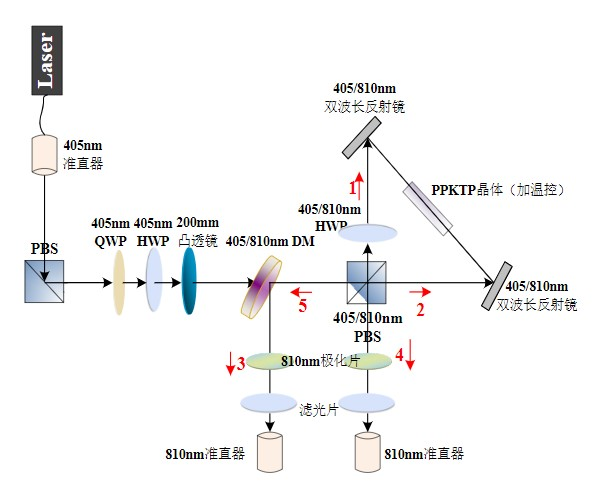
\includegraphics[width=0.9\textwidth]{./fig2.jpg}
        \caption{实验装置示意图}
    \end{minipage}
\end{figure}

 将 PPKTP 晶体和 Sagnac 环结合,即可产生高亮度的偏振纠缠源,下面给出详细分析. 泵浦光被由极化分束器(PBS)反射只剩下 V 分量,再由半波片将 V 极化的泵浦光置于 45°极化,之后再次入射极化分束器(PBS), H 分量透射,V 分量反射.透射部分直接进入 PPKTP 晶体,以一定概率打出一对信号光(H)和闲频光(V), 经 45 度半波片后极化翻转,分别记为$|V_s\rangle$和$|H_i\rangle$; 反射部分泵浦光经过 45 度半波片变换为 H, 同样以一定概率打出一对信号光(H)和闲频光(V), 分别记为$|H_s\rangle$和$|V_i\rangle$.透射和反射的泵浦光由于光强相同,所以泵出一对光子的概率也相同.透射(反射)泵浦光所产生的下转换光子分别沿Sagnac 环逆时针(顺指针)再次进入 PBS, 经 PBS 变换,信号光进入路径 3, 闲频光进入路径 5, 记为$|V_s\rangle_3|H_i\rangle_5(|H_s\rangle_3|V_i\rangle_5)$.由于光子的全同性,当在 3 和 5 端口观测到符合计数时,我们无法分辨下转换光子的顺(逆)时针,此时在 3 和 5 路径上,两个光子便处于纠缠态

$$
|\Psi^{+}\rangle_{35}=\frac{1}{\sqrt{2}}\left(\left|V_{s}\right\rangle_{3}|H_{i}\rangle_{5}+\left|H_{s}\right\rangle_{3}|V_{i}\rangle_{5}\right).
$$

这里我们可以看到,进入路径 3(5)的光子均为信号(闲频)光,这样的 Sagnac 结构能够避
免由于光谱不同产生的纠缠干涉对比度下降. 另外由于Sagnac 干涉环的两臂重合,故此结构能够保证即便较长距离的干涉,光子的波包也能较好的重合.

\subsection{实验步骤}

\begin{enumerate}
    \item 开启激光器电源,钥匙旋转至ON使激光器出光,调节功率至030.
    \item 打开符合计数器,将模式切换至符合计数.首先将两个偏振片置于90/0以及0/90,观察HV和VH的计数,并记录.
    \item 将两个偏振片分别置于$\pm 45^{\circ}$的四种组合,调节前端405nm四分之一波片和半波片,
    使得偏振片均为$+45^{\circ}$和均为$-45^{\circ}$时符合计数为大值,两偏振片角度不同时为小值,
     两大值和/两小值和应当大于10. 固定这两个拨片的度数.
    \item 根据CHSH不等式, 测量所需的符合计数, 观察并记录, 计算实验结果以及标准偏差,以三倍标准偏差违背不等式
    \item 测量关联曲线,将其中一个偏振片置于0和45度,旋转另一个偏振片,测量两条关联曲线(每条曲线间隔10度取一个点,即19个点)
    \item 关闭探测器;激光器功率调至最小,之后将钥匙置于off, 关闭电源
\end{enumerate}

\end{document}